\subsection{Seasonality}
\label{subsec:seasonality}

It is widely acknowledged that the transmission of SARS-CoV-2 is subject to seasonal
influences. Infectiousness is increased in winter when most contacts take place inside
and the immune system is weakened by low levels of vitamin D, dry air and large
temperature swings. For a detailed overview of possible drivers see
\cite{KronfeldSchor2021}.

We follow \cite{Kuehn2020} and \cite{Gavenciak2021} in modeling seasonality in the
transmission of SARS-CoV-2 as a multiplicative factor on infection probabilities. The
factor follows a sine curve that reaches its maximum at January 1 and its minimum
on June 30.

For simplicity we normalize the factor to reach one at its maximum. Thus, the formula of
the seasonality factor is given by:

\begin{equation}
\label{eq:seasonality}
    s_{c, t} = 1 + 0.5 \kappa_c  sin \left ( \pi  \left (\frac{1}{2} + \frac{t}{182.5}\right ) \right ) - 0.5 \kappa_c
\end{equation}

Where $\kappa_c$ is difference in the seasonality factor between peak infectiousness
and lowest infectiousness.

The subscript $c$ is needed because the strength of the seasonality effect differs
across contact types: Work, household and school contacts are likely to take place
inside even in summer. Thus they are only subject to seasonality due to factors that
influence the immune system. Other contacts (for example meeting friends and while doing
leisure activities) are mostly happening outside in the summer. Therefore, transmission
via those contacts should have a stronger seasonal pattern.

We calibrate $\kappa_{strong}$ to 0.42 and $\kappa_{weak}$ to 0.21. This is in line with
\cite{Gavenciak2021} and \cite{Kuehn2020}.

The two seasonality curves are shown in Figure~\ref{fig:seasonality}.

\begin{figure}
    \centering
    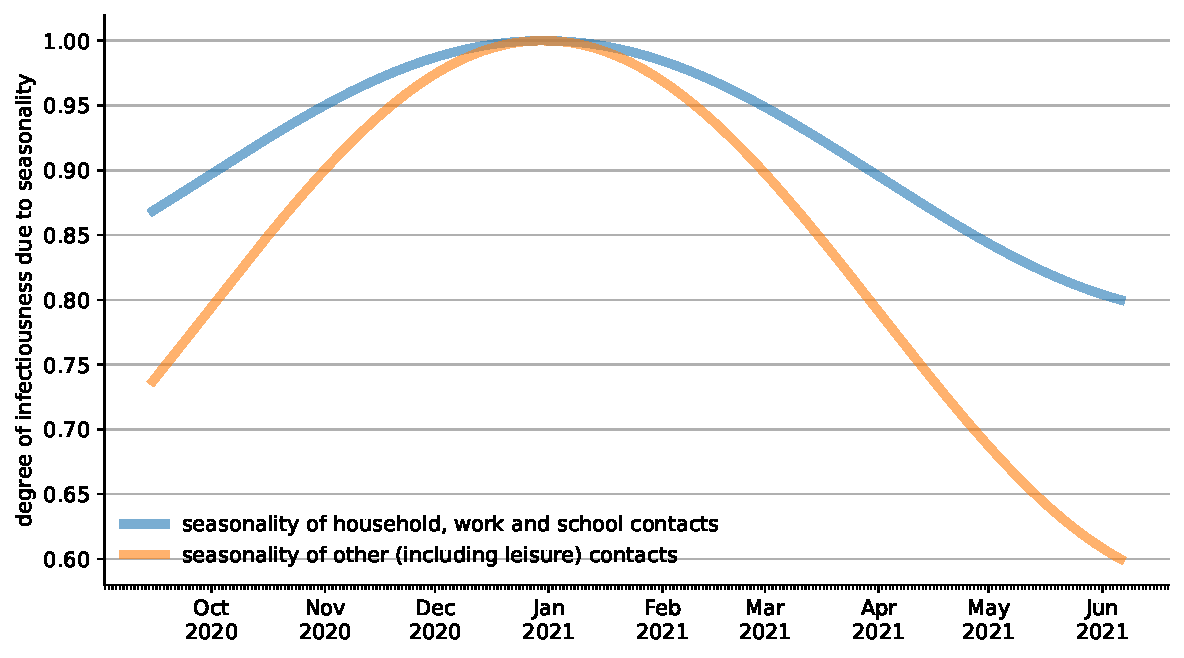
\includegraphics[width=0.5\textwidth]{figures/results/figures/data/seasonality}
    \caption{Seasonality by Type of Contact}
    \label{fig:seasonality}
    \floatfoot{\noindent \textit{Note:} We model seasonality as a factor that reduces the
    probability of infection of all encounters. The factor depends on the day and is
    calculated from a sinus shaped function with its maximum on January 1. Since
    seasonality can affect the transmission both through physical conditions such as
    temperature and humidity as well as through the numbers of contacts that take place
    outside we assume two seasonality factors. One for other contacts which we expect to
    be strongly affected by fairer weather with a maximum reduction of 42\% in the
    infection probability. The other seasonality only makes contacts up to 21\% less
    infectious and is applied to household, work and school contacts.}
\end{figure}

\FloatBarrier
